\section{Coletas de Dados com os Pacientes}

% ********************** FALAR DO COMITE DE ÉTICA *************************  
% - TAMANHO DA AMOSTRAGEM / LOCAL DE COLETA - Falar do LIS / falar da especialista / explicitar que esta fase vai para dentro do software / Acrescentar anexo (ficha, tcle) e apendice (doc visao e arquitetura) / 

    As coletas de dados foram implementadas seguindo uma estrutura de ficha, definida a partir das normas de avaliação CIF. Sendo assim, todas as coletas de dados seguiram a ordem conforme a Figura 10. 

    \begin{itemize}
        \item Acolhimento do paciente e coleta de seus dados pessoais;
        \item Aplicação da ficha de avaliação do paciente, feita por um profissional da área de saúde;
        \item Sessão de fotos do coto e do paciente para futura análise postural e de condição da pele.
    \end{itemize}

    A ficha de avaliação aplicada junto ao paciente pelo profissional da saúde é um dos produtos de \textit{software} desenvolvidos para facilitar e agilizar a avaliação do paciente.

    \begin{figure}[ht]
        \centering
        \label{fig10}
            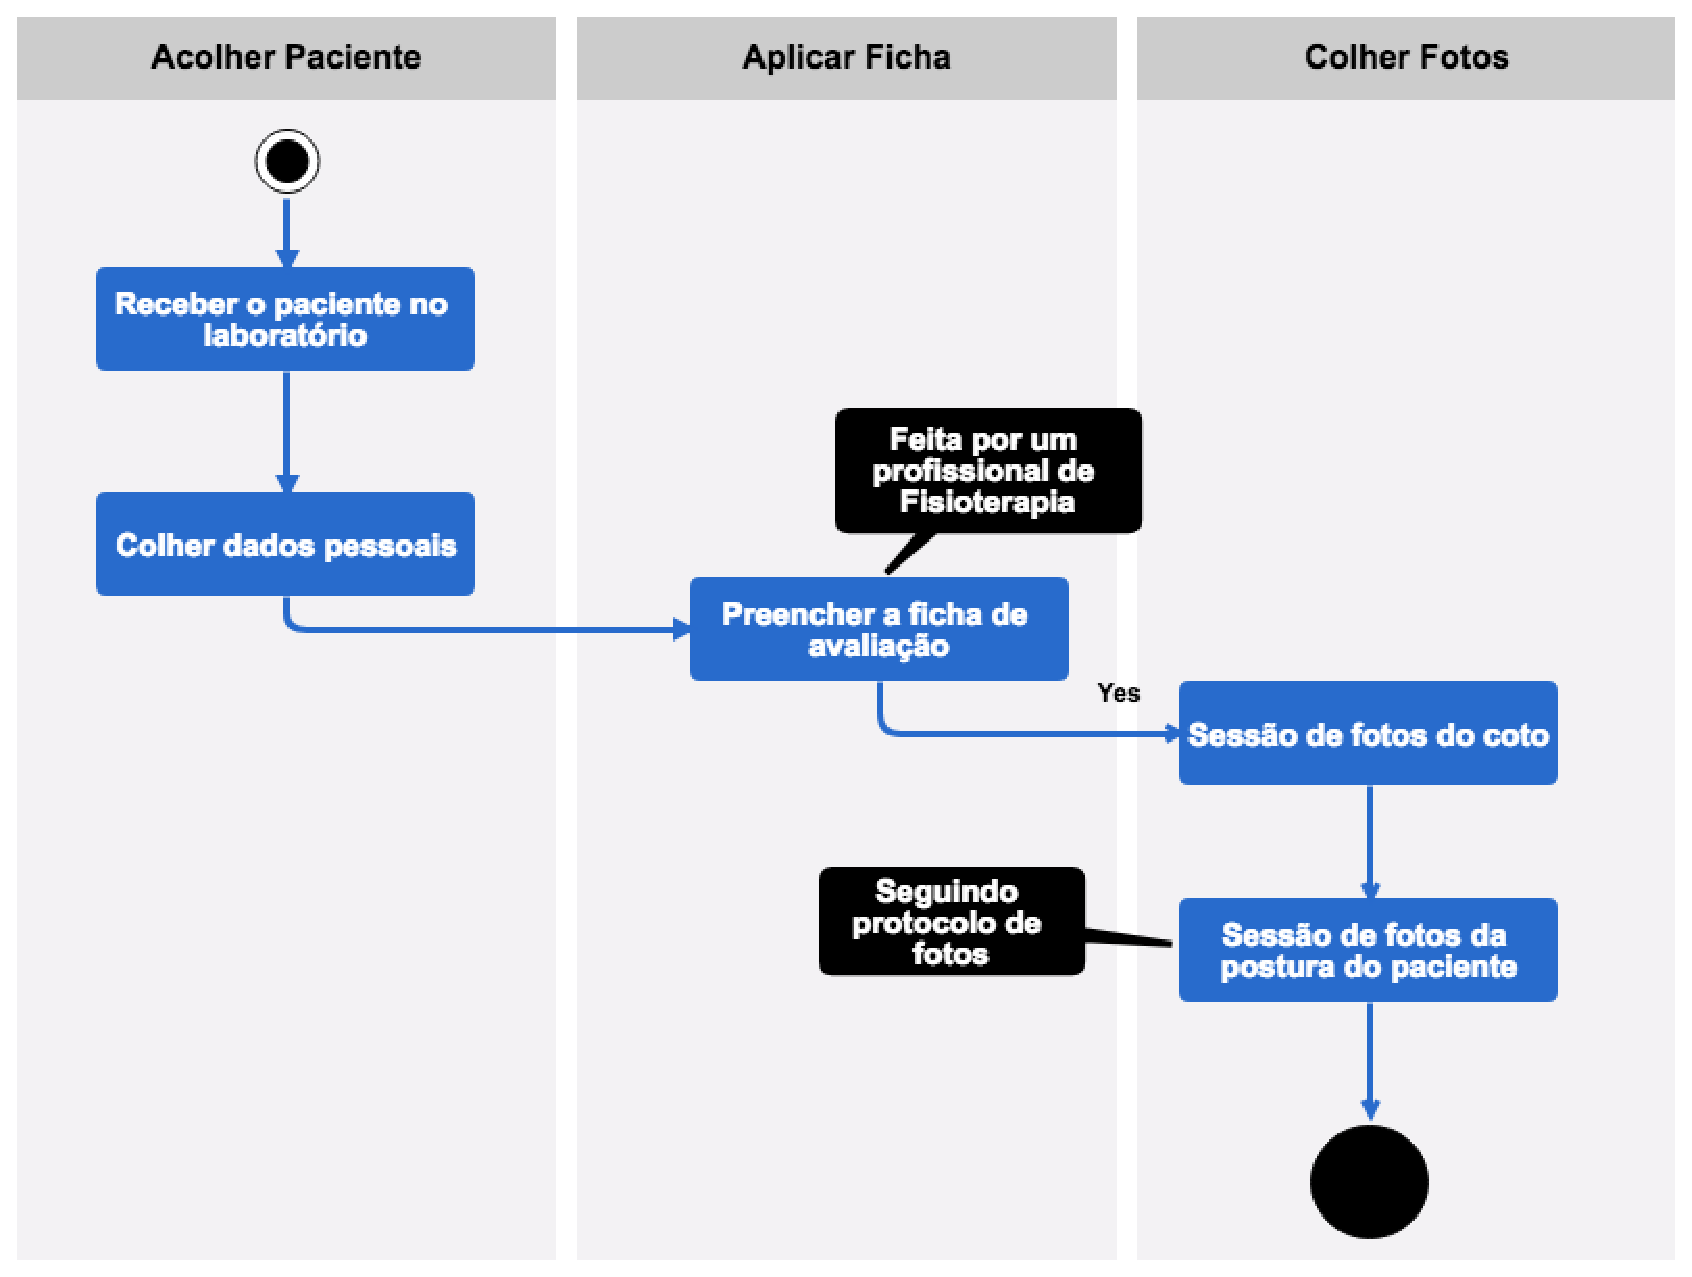
\includegraphics[keepaspectratio=true, scale=0.4]{editaveis/images/colet_flow.eps}
        \caption{Fluxo de trabalho da coleta}
    \end{figure}

    A sessão de fotos do coto do paciente foi realizada para ser o mais simples possível, para que todo profissional da área da saúde possa conseguir coletar este dado sem necessidade de conhecimento técnico de fotografia ou de um protocolo rígido. O profissional da saúde precisa apenas de uma câmera fotográfica, ou celular com câmera, para fazer o registro com a única restrição de que a imagem gerada seja completamente preenchida pela pele do paciente. As fotografias devem ser tiradas de todos os lados do coto, tais como sua frontal, posterior, laterais interna e externa e por último da vista da amputação (cicatriz).

    Para que pudessem ser feitas as coletas de dados de pacientes, foi necessário um Comitê de Ética e Pesquisa (CEP), o qual disponibilizou a autorização com o número CAAE 38386714.8.0000.0030 (Anexo C). Foram feitas coletas com 13 pacientes amputados de membro inferior diferentes no decorrer da pesquisa, todas com o auxílio de uma fisioterapeuta especialista na área de tratamento com pacientes amputados. Os tipos de pele dos 13 pacientes coletados são descritos na Tabela 1.

    \begin{table}[H]
            \centering
            \label{tab01}
            \caption{Descrição da quantidade de cada tipo de pele dos cotos.}
            \begin{tabular}{|l|l|}
                \hline
                Tipo de Pele & Quantidade \\ \hline
                Normal       & 9          \\ \hline
                Pálido       & 3          \\ \hline
                Cianótico    & 1          \\ \hline
            \end{tabular} 
        \end{table}

    Os dados foram coletados, em sua maioria, no Laboratório de Análise de Movimento e Processamento de Sinais da Faculdade da Ceilândia da Universidade de Brasília (FCE-UnB), apesar de terem ocorrido casos em que a coleta foi feita na casa do paciente, trabalhando em conjunto com o centro da pesquisa que foi o Laboratório de Informática em Saúde (LIS) da Faculdade Gama da Universidade de Brasília (FGA-UnB). 


    % \begin{figure}[ht]
    %     \centering
    %     \label{fig08}
    %         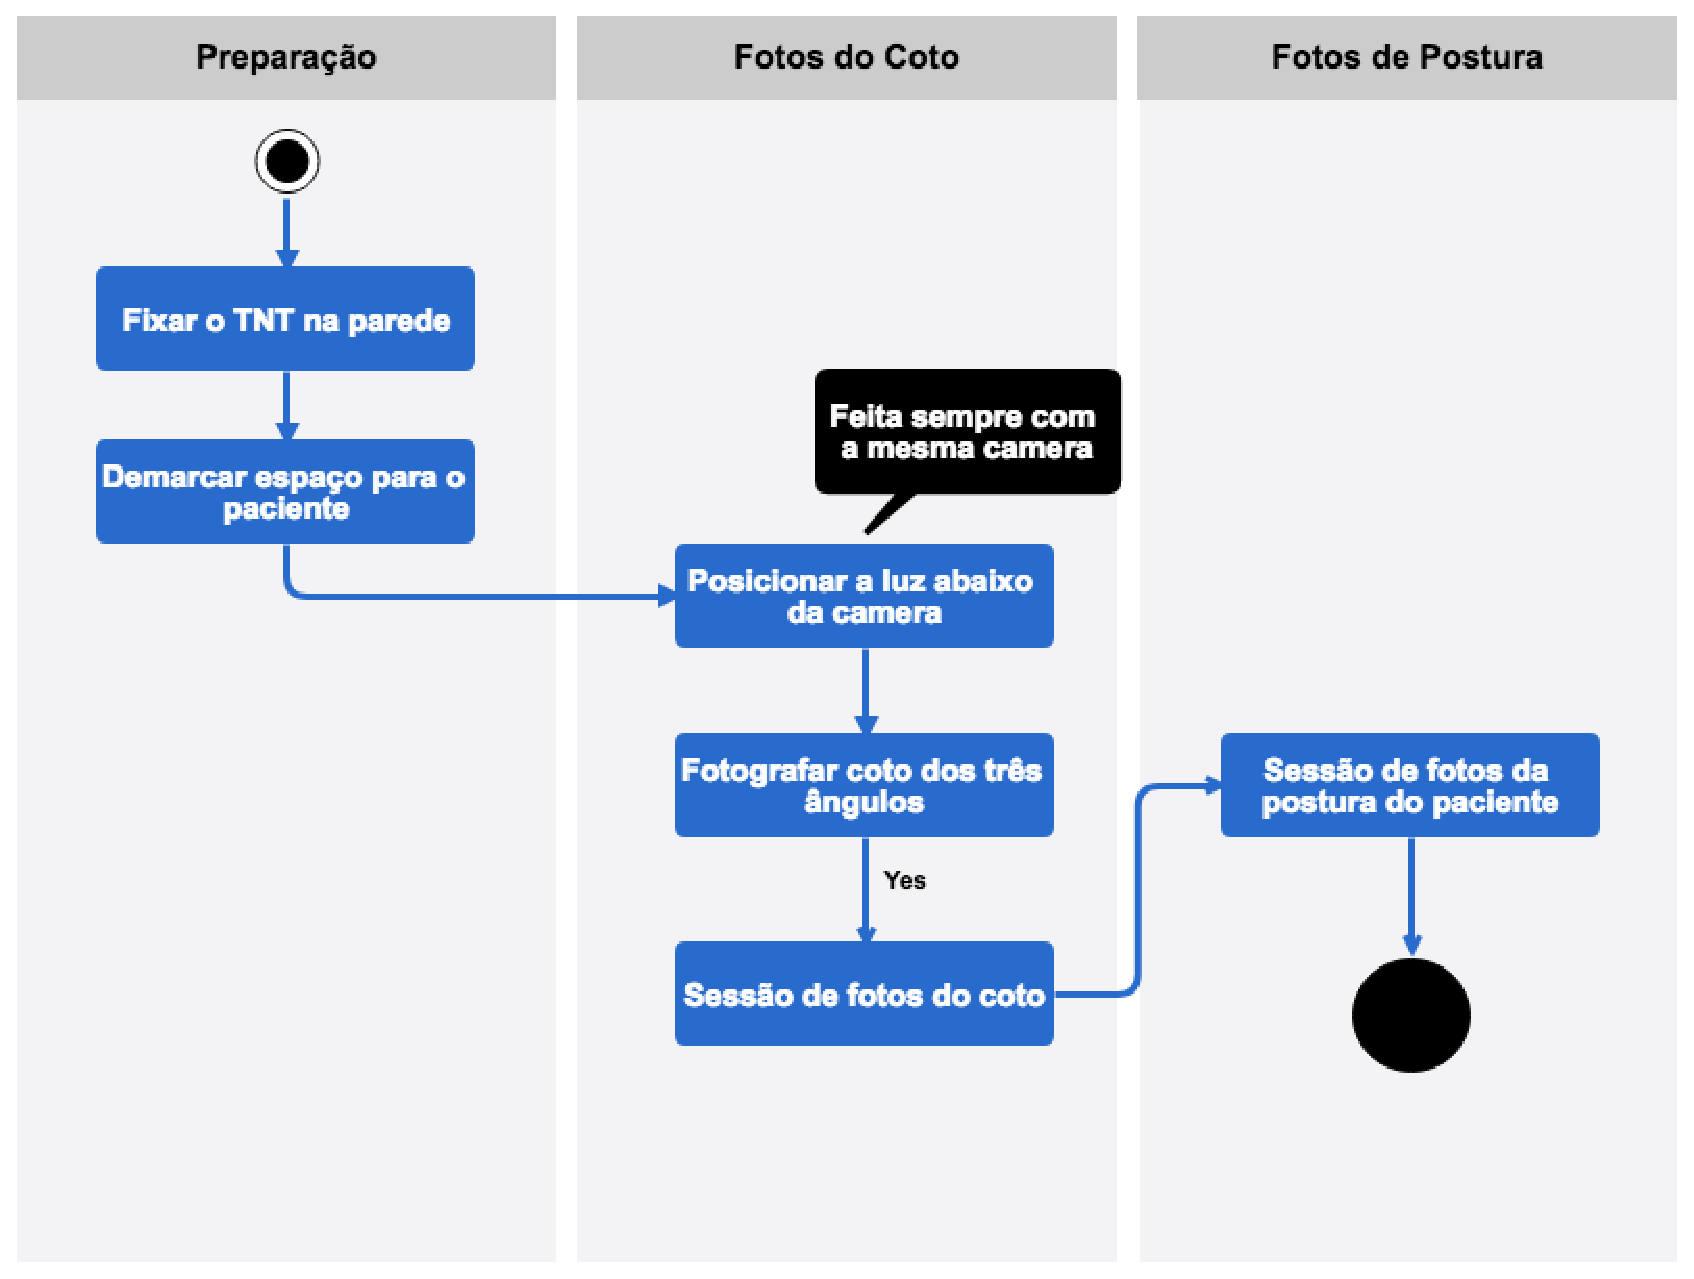
\includegraphics[keepaspectratio=true, scale=0.4]{editaveis/images/fotos_flow.eps}
    %     \caption{Fluxo de trabalho das fotografias}
    % \end{figure}

\section{Software GPSATWeb}
    % ******************** DESCREVER SIGLA GPSAT **********************
    O \textit{software} GPSATWeb, assim denominado pois nasceu das ações do Grupo de Pesquisa sobre Saúde de Amputados Transfemorais e Tecnologias (GPSAT), foi construído utilizando a interação de dois sistemas separados, um \textit{web} para interação com o usuário e uma \textit{api restful} que trabalha com as requisições de todos os dados do sistema. O modelo construído é apresentado na Figura 11 e descrito no documento de visão (Apêndice A). 

     \begin{figure}[ht]
        \centering
        \label{fig11}
            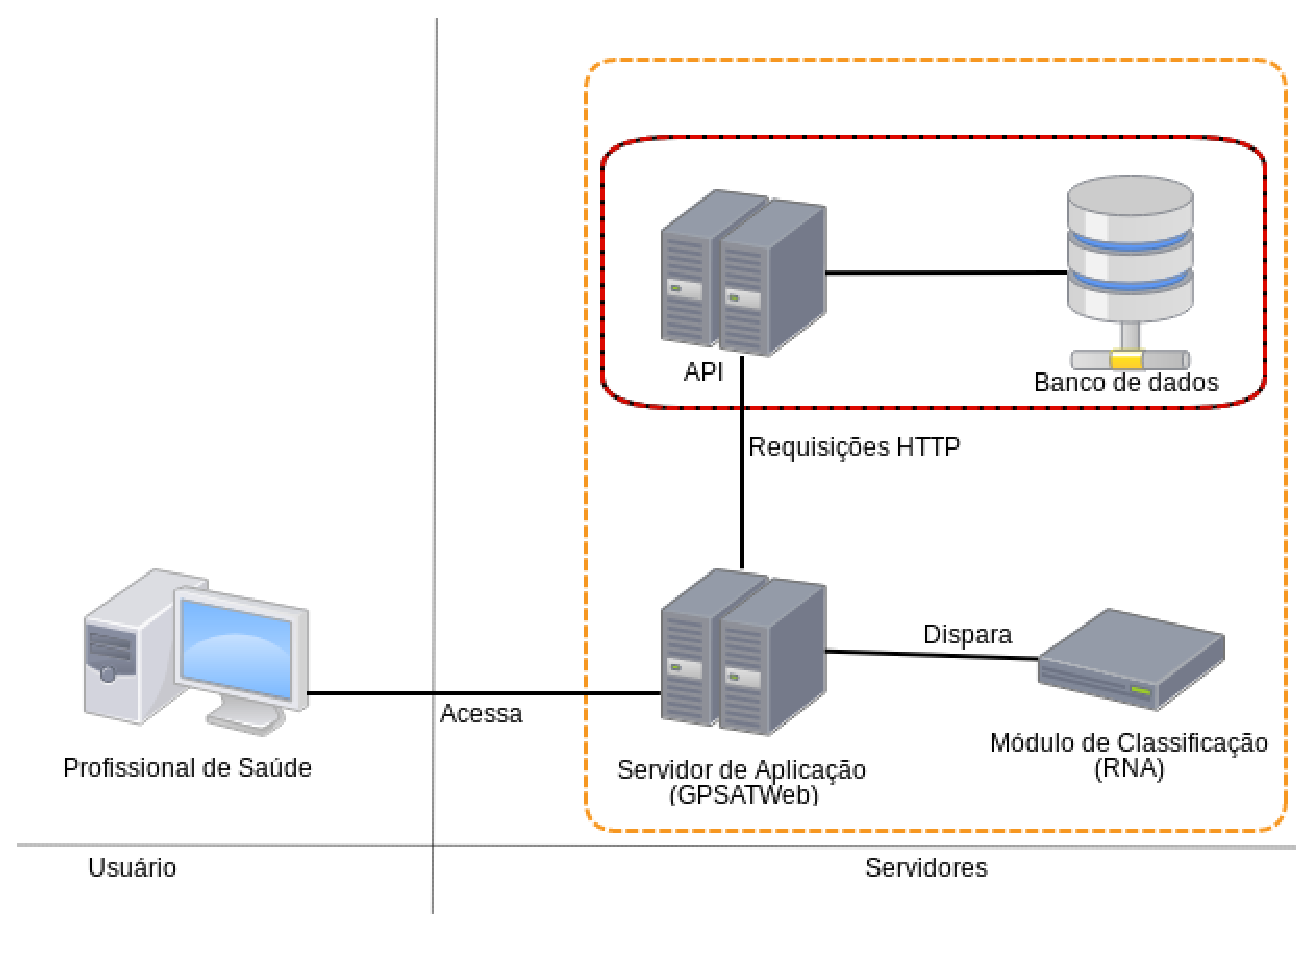
\includegraphics[keepaspectratio=true, scale=0.6]{editaveis/images/arquiteturaGPSATWeb.eps}
        \caption{Disposição dos componentes da aplicação.}
    \end{figure}

    \subsection{Web}
        O \textit{software} GPSATWeb foi construído utilizando a linguagem de programação \textit{Python} e o \textit{framework} Django. Este \textit{framework} implementa o padrão de arquitetura \textit{Model-View-Controller} (MVC).

        O padrão de arquitetura MVC é dividido em três camadas: modelo, visão e controlador. Cada uma destas camadas é responsável por uma atividade dentro do sistema. Quais sejam \cite{Lemos2013}:
            \begin{itemize}
                \item Modelo: Camada em que acontece a presistência dos dados do sistema em uma base de dados. Somente nesta camada as quatro operações básicas de um banco de dados, isto é, criação, edição, leitura e atualização de dados podem ocorrer;
                \item Visão: Camada de interação com o usuário. É nela que todos os dados sao mostrados e recebidos;
                \item Controlador: Camada que controla todo o fluxo do sistema. Nesta camada é feita a comunicação entre outras duas, a da visão e a de modelo. Além disso, nesta camada ocorre o processamento de todos os dados, tanto de entrada quanto de saída do sistema.
            \end{itemize}

        No caso do GPSATWeb, a camada modelo não interage diretamente com a base de dados, ela envia requisições HTTP com os dados a serem persistidos e o tipo de operação a ser realizada para a \textit{api}, como descrito no documento de arquitetura (Apêndice B). 
        
    \subsection{API Restful}
        A \textit{api} construída é um serviço \textit{web restul} construído para receber e transmitir os dados do sistema GPSATWeb via requisições remotas, pois assim o acesso à base de dados independe de o sistema \textit{web} estar \textit{online} ou não. 

        A \textit{api} utiliza para a base de dados o MongoDb que é uma ferramenta de banco de dados orientado a documentos. Estes tipos de bancos de dados foram originalmente desenvolvidos para salvar documentos de todos os tipos, estes documentos são codificados em formatos padrões internacionais, tais como JSON ou XML. Suas vantagens, além da flexibilidade adiquirida por usar estes formatos, são segundo \cite{Moniruzzaman2013}:
        \begin{itemize}
            \item Baixa latência de resposta para leitura e escrita;
            \item Eficiência em armazenar grandes quantidades de dados;
            \item Alta escalabilidade.
        \end{itemize}

\section{Modelo de Machine Learning}

    Tendo como meta a definição de um modelo de ML para ser aplicada em uma RNA a ser treinada para detecção de tipos de pele, a estratégia a ser seguida foi o fluxo de trabalho de ML, descrito na Figura 6 e adaptado para esta aplicação como mostra a Figura 12.

    \begin{figure}[ht]
        \centering
        \label{fig12}
            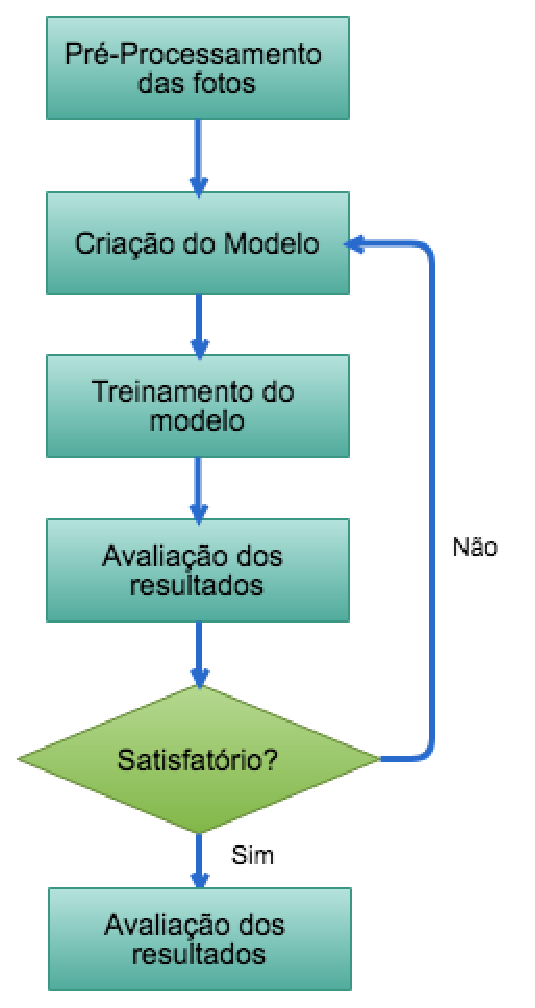
\includegraphics[keepaspectratio=true, scale=0.6]{editaveis/images/ml_nt_flow.eps}
        \caption{Fluxo de trabalho da construção do modelo de ML}
    \end{figure}

    \subsection{Construção do Modelo}

        O modelo de aprendizado utilizado foi o supervisionado, baseado em uma RNA MLP com método de treinamento \textit{backpropagation}.
        Sendo assim, os passos a serem seguidos para a construção do modelo inicial foram:

        \begin{itemize}
            \item Pré-processamento dos dados \\ Neste primeiro passo, é montado o modelo de dados de treinamento que é usado para apresentação e utilização dos dados. Para isso é necessário encontrar uma correlação entre os dados de entrada e o dado a ser atingido pelo processo de aprendizado.

            \item Criar o modelo \\ O modelo deve ser criado para receber os dados de entrada como pré-processados para fazer seu processamento visando o resultado a ser obtido.

            \item Treinar o modelo \\ O modelo proposto deve passar por um breve treinamento para que os erros sejam corrigidos antes que a RNA comece a receber dados para serem analisados.

            \item Avaliar o modelo \\ Uma vez com o modelo pronto é necessário avaliar a aplicabilidade do modelo em vista da acurácia obtida em relação a quantidade de reconhecimentos feitos em uma base de dados controlada e com um número conhecido de dados coletados dos pacientes.

            \item Apresentar resultados \\ Assim que o modelo é avaliado, se for julgado com resultado insatisfatório, ele deve ser reencaminhado para uma melhoria na modelagem. Caso seja satisfatório, devem ser apresentados aqui os resultados obtidos.
        \end{itemize}
